\documentclass[main.tex]{subfiles}

\begin{document}

\chapter{Класична аналогија ЕИТ-а}%
\label{cha:klasik_eit}

\section{Увод}%
\label{sec:uvod}

У ласерској физици, електромагнетно-индукована транспаренција (ЕИТ) је ефекат у којем се, у оквиру апсорпционе линије медијума, јавља веома узак опсег транспаренције. Типично се ради о системима са три нивоа, између којих је остварена одговарајућа кохеренција помоћу два ласерска снопа. Ефекат је пропраћен израженом дисперзијом, која доводи до тзв. „споре светлости``~\cite{harris1990nonlinear}.

Често су вршена истраживања класичних аналогија одређених квантних ефеката, нпр. тунеловање у таласоводима, тополошки изолатори (швец), силвериња се исто нешто бавио тиме... % допуни са референцама!!!
У случају ЕИТ-а, показује се да постоји формална сличност са спрегнутим класичним осцилаторима~\cite{garrido2002classical}. Одговарајућа спрега између осцилатора може се реализовати у различитим системима, као што су нпр. спрегнути механички/електрични осцилатори, при чему је ефекат познат под називом \emph{класична аналогија ЕИТ-а}.%За остваривање, потребно је имати два или више резонатора, који су различито спрегнути са спољашњом побудом – слабо спрегнути, тзв. тамни елемент, са великим $Q$-фактором, и јако спрегнути, тзв. светли елемент, са ниским $Q$-фактором.

Од посебног интереса је реализација класичног ЕИТ-а у метаматеријалима који са спрегнутим резонаторима. Ефекат се манифестује као оштар трансмисиони максимум у оквиру апсорпционе линије~\cite{tassin:09,cihan,mr05}. Пропраћен је наглашеном дисперзијом, која резултује високом вредношћу групног кашњења, односно малом групном брзином. Измерене су вредности више од 200 пута спорије пропагације таласа него у слободном простору, што чини ову врсту метаматеријала погодним за примене са успоравањем светлости у терахерцном опсегу~\cite{tassin:09}, као и за линије за кашњење у микроталасном опсегу~\cite{mr05}. Такође, због високог $Q$-фактора и израженог конфинирања поља, резонантни максимум је веома осетљив на промене индекса преламања у окружујућој средини, што је пожељно за сензорске примене.

\section{Интеракција атома са ласерским зрачењем}

Најпре ће бити размотрен најједноставнији случај атома у пољу резонантног ласерског зрачења. Користиће се семикласична анализа, у којој је атом представљен као квантни систем са два нивоа, основним стањем, $\ket{1}$, и побуђеним стањем, $\ket{2}$. Претпоставка је да су стања различите парности, тако да је дозвољен диполни прелаз између њих, са фреквенцијом $\omega_{21}$. С друге стране, ЕМ талас се третира на класичан начин преко Максвелове теорије. За монохроматско електрично поље $E = E_0\cos{\omega_L t}$, Хамилтонијан интеракције износи $H_{int} = E_0\mu_e\cos{\omega_L t}\dyad{2}{1}$, где је $\mu_e = \mel{2}{\hat{d}}{1}$ матрични елемент оператора електричног дипола, паралелан пољу~\cite{suter1997physics}. Уобичајено се користи апроксимација ротирајућег таласа (\foreign{rotating wave approximation}), уз одговарајућу трансформацију базиса, како би се отклонила временска зависност интеракције. У том случају укупни Хамилтонијан система има облик:
\begin{equation}
    \label{eq:ham2}
    H = \hbar \left\{ -\delta_p\dyad{2} - \frac{1}{2}\Omega_p\dyad{2}{1} + \textit{х.к.} \right\},
\end{equation}
где је $\delta_p = \omega_{21} - \omega_L$, а $\Omega_p = E_0 \mu_e$ представља фреквенцију Рабијевих осцилација. Сада се може добити временска зависност матрице густине као:
\begin{equation}
    \dot \rho = -\frac{i}{\hbar}\left[ H,\rho \right] + слабљење,
\end{equation}
на основу чега се за елемент матрице $\rho_{21}$ добија~\cite{xu2010studies}:
\begin{equation}
    \label{eq:ro211}
    \dot \rho_{21} = \frac{i}{2}\Omega_p (\rho_{11} - \rho_{22}) + i\delta_p \rho_{21} - \gamma_{21}\rho_{21}.
\end{equation}
Израз (\ref{eq:ro211}) може се упоредити са класичним осцилатором, као што је честица на крају еластичне опруге, или резонантно $LC$ коло, под дејством спољашње силе. У том случају, $\delta_p$ одговара сопственој резонантној учестаности, $\gamma_{21}$ представља коефицијент губитака, а члан који садржи Рабијеву фреквенцију одговара спољној побуди.

%%%%%%%%%%%%%%%%%%%%%%%%%%%%%%%%%%%%%%%%%%%%%%%%%%%%
%  не могу сад да улазим у то, гледаћу касније...  %
%%%%%%%%%%%%%%%%%%%%%%%%%%%%%%%%%%%%%%%%%%%%%%%%%%%%
%У случају честице масе $m$, која се налази на крају опруге коефицијента еластричности $k$, и под дејством спољашње силе $\vec{F}$, на основу другог Њутновог закона може се написати:
%\begin{equation}
    %m\ddot{x} = % морам још мало размислити...
%\end{equation}
\begin{figure}[h]
    \centering
    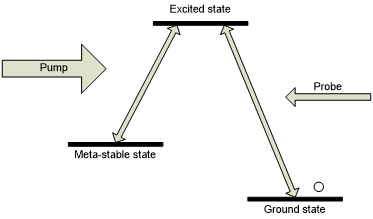
\includegraphics[width=0.8\linewidth]{sl_eit/lambda.png}
    \caption{$\Lambda$ конфигурација.}
    \label{fig:sl_eit/lambda}
\end{figure}
У случају атома са три нивоа, један од прелаза мора бити забрањен за диполе због исте парности. Претпоставимо да су прелази $\ket{1}\to\ket{2}$ и $\ket{2}\to\ket{3}$ дозвољени, а $\ket{1}\to\ket{3}$, због чега је стање $\ket{3}$ метастабилно. Уколико је прелаз $\ket{1}\to\ket{2}$ побуђен пробним ласером (\foreign{probe}), са Рабијевом фреквенцијом $\Omega_p$, а прелаз $\ket{1}\to\ket{3}$ пумпајућим ласером (\foreign{pump}), Рабијеве фреквенције $\Omega_c$, Хамилтонијан система има следећи облик:
\begin{equation}
    H = \hbar \left\{ -\delta_p\dyad{2}{2} - \delta_c\dyad{3}{3} - \frac{1}{2}\left( \Omega_p \dyad{2}{1} + \Omega_c \dyad{3}{1}\right) + \textit{х.к.}  \right\},
\end{equation}
на основу кога се добија једначина кретања за матрични елемент:
\begin{equation}\label{eq:ro212} 
    \dot \rho_{21} = \frac{i}{2}\Omega_p(\rho_{11}-\rho_{22}) + \frac{i}{2}\Omega_c\rho_{32} + i\delta_p\rho_{21} - \gamma_{21}\rho_{21}.
\end{equation}
Додатни члан у (\ref{eq:ro212}) у односу на (\ref{eq:ro211}) у контексту класичне аналогије може се интерпретирати као спрега са другим осцилатором. У случају када је детјунинг оба ласера једнак, $\delta_p = \delta_c$, показује се да постоји суперпозиција стања $\ket{2}$ и $\ket{3}$ која је потпуно неспрегнута са побудом, тзв. „тамно стање`` (\foreign{dark state, trapping state}). Приликом интеракције са пољем, атом пролази кроз циклусе апсорпције и реемисије, при чему увек постоји вероватноћа да падне у тамно стање, где након тога и остаје. После неког времена, сви атоми ће се наћи у тамном стању, и апсорпција у систему ће нестати~\cite{suter1997physics}.

\section{Модел спрегнутих осцилатора}%
\label{sec:model_spregnutikh_ostsilatora}
\begin{figure}[h]
    \centering
    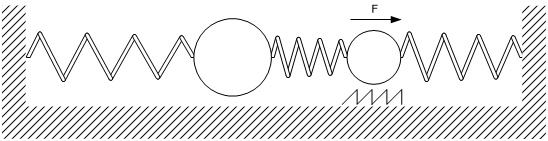
\includegraphics[width=0.8\linewidth]{sl_eit/opruge.png}
    \caption{Спрегнути механички осцилатори.}
    \label{fig:sl_eit/opruge}
\end{figure}
На сл.~\ref{fig:sl_eit/opruge} је приказан систем два спрегнута механичка осцилатора, који ће бити коришћен за објашњење механизма класичне аналогије ЕИТ-а. Претпоставимо да честице обележене са 1 и 2 имају масе $m_1$ и $m_2$, респективно. Оба осцилатора, када нису спрегнута (тј. без опруге у средини), имају исту резонантну учестаност $\omega_0$, док је константа слабљења за честицу 2 много мања него за честицу 1, $\gamma_2\ll\gamma_1$. Коефицијент спреге је $\kappa$. Онда, ако спољашња синусоидална сила делује на честицу 1, $F=F_0e^{j\omega t}$, једначине кретања имају следећи облик ($x_{1,2}$ представља растојање одговарајућих честица од њиховог равнотежног положаја):
\begin{align}
    %\label{eq:spreg_osc}
    \ddot x_1 + \gamma_1 \dot x_1 + \omega_0^2 x_1 + \kappa x_2 & = F = F_0 e^{j\omega t}, \label{eit:jkr1} \\
    \ddot x_2 + \gamma_2 \dot x_2 + \omega_0^2 x_2 + \kappa x_1 & = 0.\label{eit:jkr2}
\end{align}
%\begin{align}
    %%\label{eq:spreg_osc}
    %\frac{\partial^2x_1}{\partial t^2} + \gamma_1 \frac{\partial x_1}{\partial t} + \omega_0^2 x_1 + \kappa x_2 & = F = F_0 e^{j\omega t}, \label{eit:jkr1} \\
    %\frac{\partial^2 x_2}{\partial t^2} + \gamma_2 \frac{\partial x_2}{\partial t} + \omega_0^2 x_2 + \kappa x_1 & = 0.\label{eit:jkr2}
%\end{align}
%У овој аналогији, сила $F$ представља упадни талас чија трансмисија се мери (пробни талас), ... ПРОВЕРИ АНАЛОГИЈУ (ПОШТО ОВО КАКО ЈЕ НАВЕДЕНО НИЈЕ ТАЧНО)!!

Кретање честице 1 је повезано са апсорпцијом због трења; уколико ова честица мирује, апсорпција неће бити присутна. Решавањем система (\ref{eit:jkr1})–(\ref{eit:jkr2}) добија се следећи израз за померај:
\begin{equation}
    \label{eq:pomeraj}
    x_1 = \frac{\left( \omega_0^2 - \omega^2 + j\omega\gamma_2 \right)F_0}{\kappa^2 + \left( \omega_0^2 - \omega^2 + j\omega\gamma_1 \right) \left( \omega_0^2 - \omega^2 + j\omega\gamma_2   \right)}.
\end{equation}
Из (\ref{eq:pomeraj}) се види да је померај прве честице, на резонантној учестаности $\omega_0$, пропорционалан константи слабљења друге честице, $\gamma_2$, за који је претпоставка да је веома мали, због чега је и апсорпција такође мала. У граничном случају $\gamma_2\to 0$, очигледно је да $x_1$ такође тежи нули, дакле апсорпција у систему је у потпуности уклоњена.

Један од првих покушаја реализације класичне аналогије ЕИТ-а помоћу спрегнутих резонатора у метаматеријалима дата је у реф.~\cite{tassin:09}. Коришћени су сплит рингови са асиметричним процепима, или асиметрично постављени у односу на спољашње поље, како би се обезбедила асиметрична побуда. Такође су коришћени диелектрици са различитим тангенсом губитака, како би се остварила потребна разлика у факторима доброте. Остварена је вредност групног индекса око 100, уз истовремено веома мале губитке у трансмисији. Други рад истих аутора користи другачији приступ, са различитим врстама резонатора (сплит ринг и кратке жице), како би се остварила разлика у $Q$-факторима~\cite{tassin2009planar}. Како би се избегла ограничења због губитака у металима, предложено је коришћење суперпроводних ниобијумских (Nb) филмова~\cite{cihan}. Додатна предност овог приступа је могућност укључивања/искључивања ефекта регулацијом температуре.

\section{Аналогија ЕИТ-а побуђена водом}%
\label{sec:analogija_eit_a_pobudjena_vodom}

\begin{figure}[h]
    \centering
    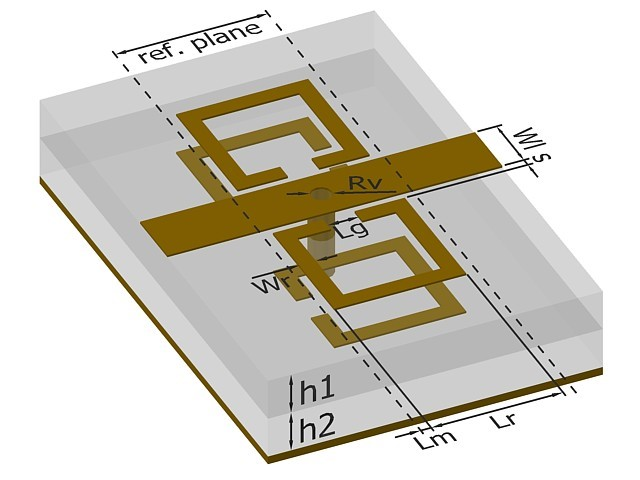
\includegraphics[width=0.8\linewidth]{sl_eit/jc2.jpg}
    \caption{Димензије: $h_1=\SI{0.635}{\milli\meter}$, $h_2=\SI{1.575}{\milli\meter}$, $\varepsilon_{r1}=\num{10.2}$, $\varepsilon_{r2}=\num{2.2}$, $L_r=\SI{3.15}{\milli\meter}$, $L_m=\SI{0.25}{\milli\meter}$, $L_g=\SI{0.75}{\milli\meter}$, $S=\SI{0.2}{\milli\meter}$, $W_1=\SI{1.4}{\milli\meter}$, $W_2=\SI{0.4}{\milli\meter}$, $W_3=\SI{0.5}{\milli\meter}$}
    \label{fig:sl_eit/jc2}
\end{figure}
У свим претходним примерима класичне аналогије ЕИТ-а, систем је побуђиван раванским таласима или помоћу таласовода. У наставку ће бити приказан случај побуде водом, приказан у~\cite{mr03:eit}. Геометрија је дата на сл.~\ref{fig:sl_eit/jc2}, где су прстенови у средњем слоју заротирани за \SI{90}{\degree} у односу на уобичајену конфигурацију, како би се обезбедила асиметрична побуда.

\begin{figure}[h!]
    \centering
    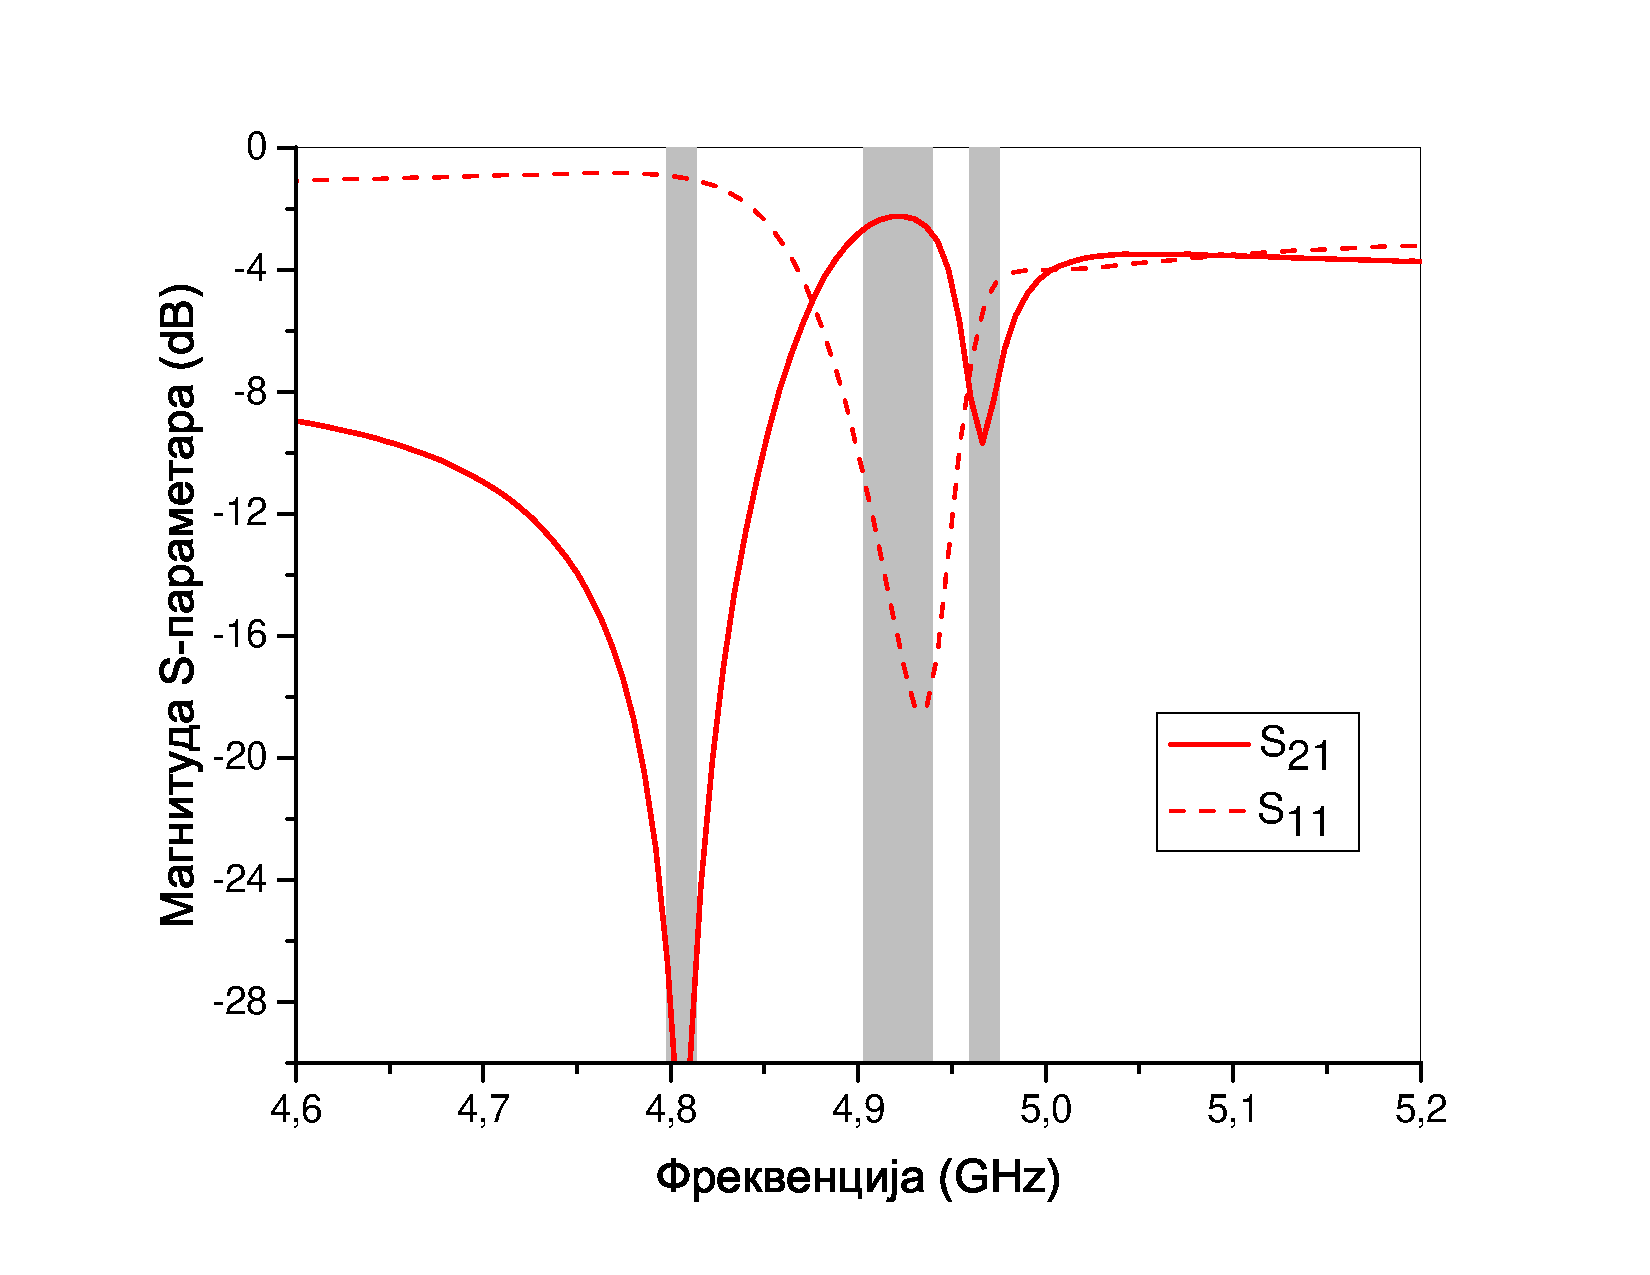
\includegraphics[width=0.8\linewidth]{sl_eit/mag.pdf}
    \caption{Спектар симулираних параметара расејања.}
    \label{fig:sl_eit/mag}
\end{figure}
\begin{figure}[h!]
    \centering
    \subfloat[]{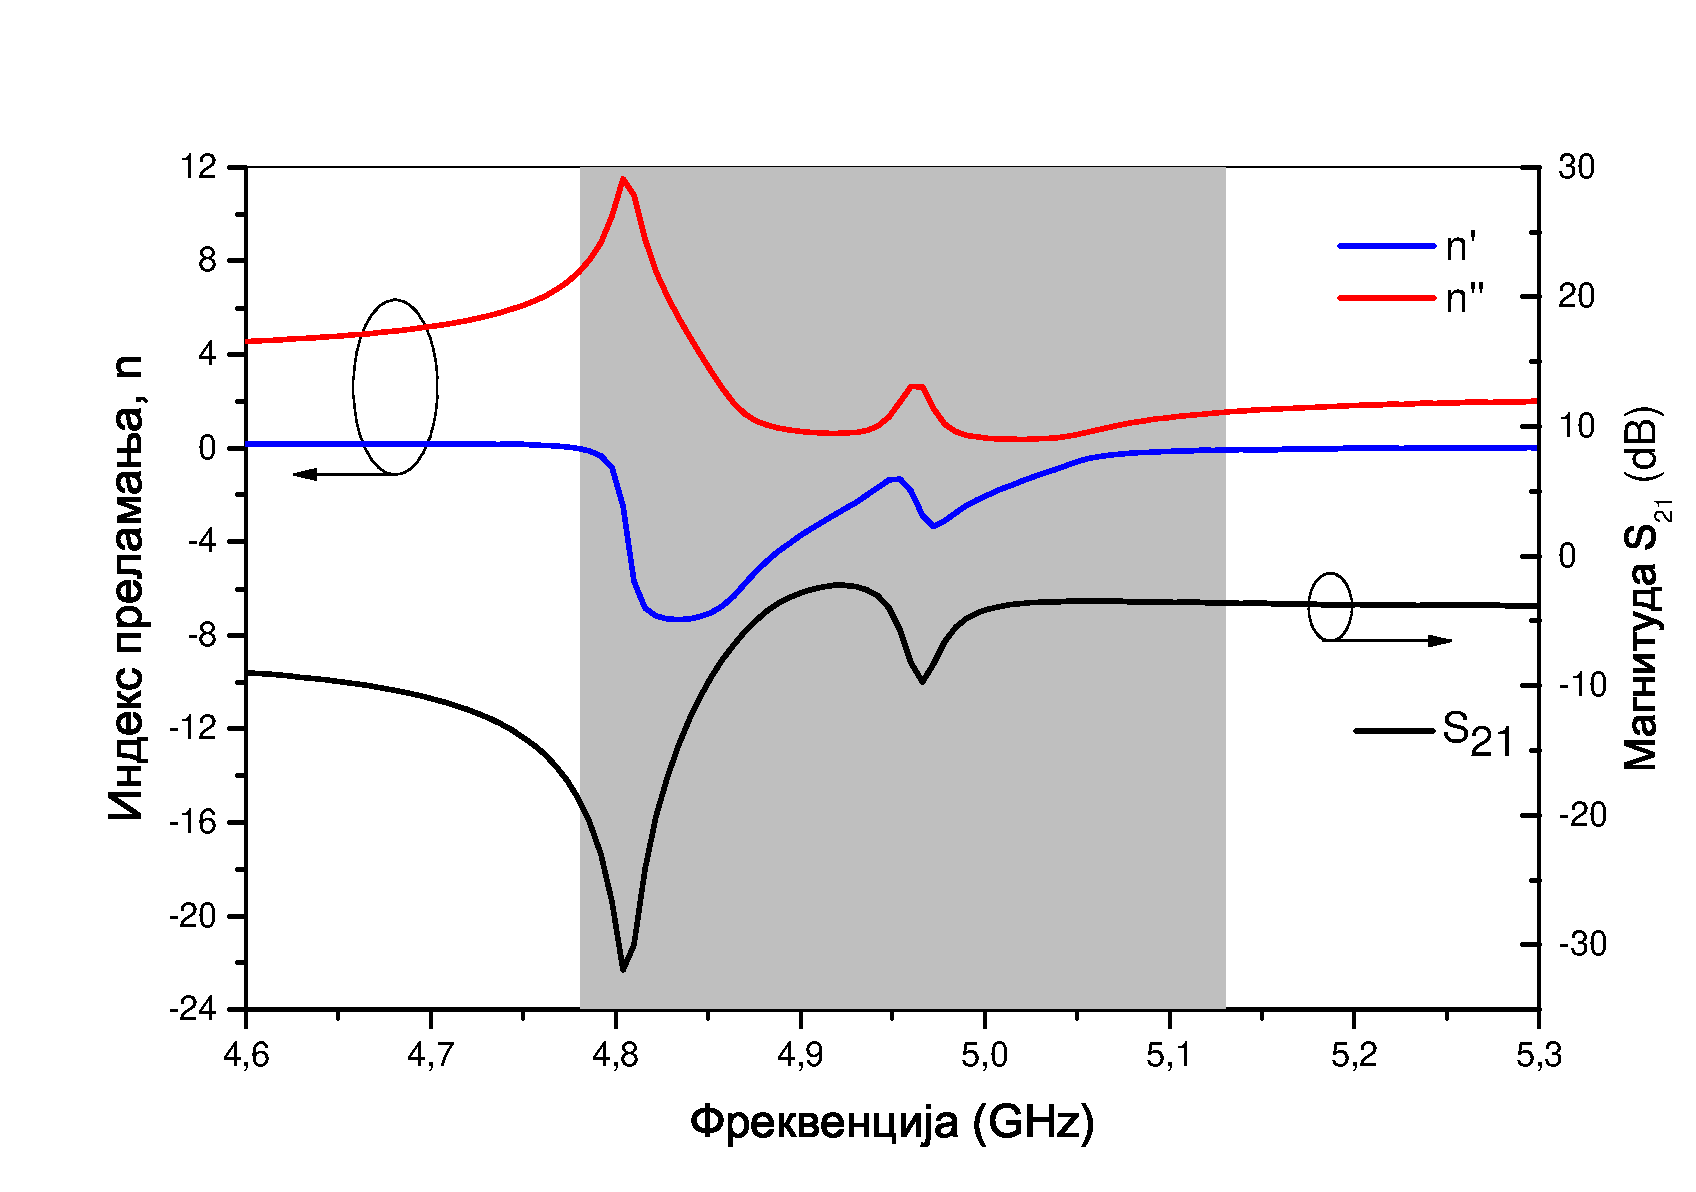
\includegraphics[width=0.9\linewidth]{sl_eit/n2.pdf}}\\
    \subfloat[]{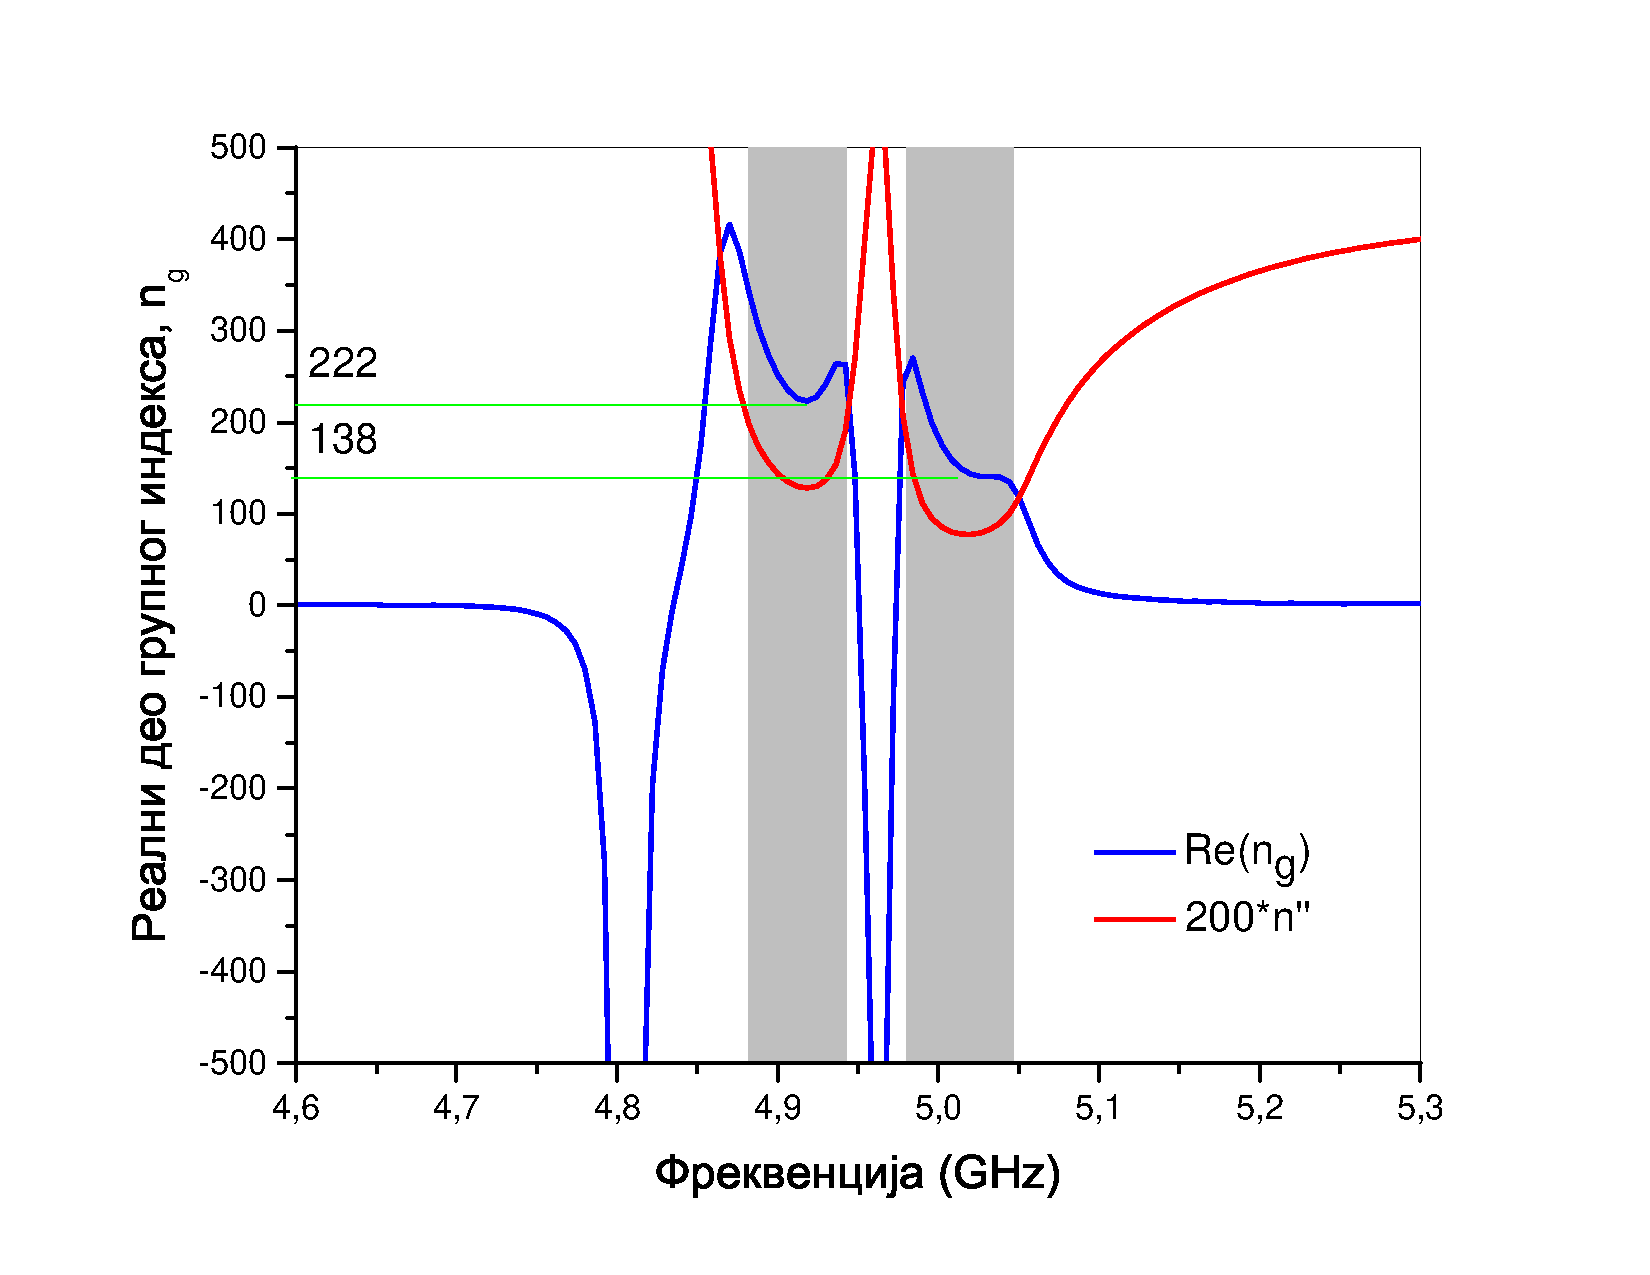
\includegraphics[width=0.9\linewidth]{sl_eit/gn2.pdf}}
    \caption{Екстраховани индекс преламања (а) и групни индекс (б).}
    \label{fig:indeksi}
\end{figure}
Симулирани спектар приказан је на сл.~\ref{fig:sl_eit/mag}, где се види присуство трансмисионог максимума, окруженог апсорпционим резонансама са обе стране (осенчени делови на графику). Даље је екстрахован ефективни индекс преламања, на основу кога је прорачунат групни индекс према формули $n_g = n + \omega(\nicefrac{\partial n}{\partial \omega})$, и добијени резултати су приказани на сл.~\ref{fig:indeksi}. Максимална вредност групног индекса износи око 220, што је за ред величине веће него у случају када прстенови нису заротирани ($\approx 25$).

\begin{figure}[h!]
    \centering
    \subfloat[]{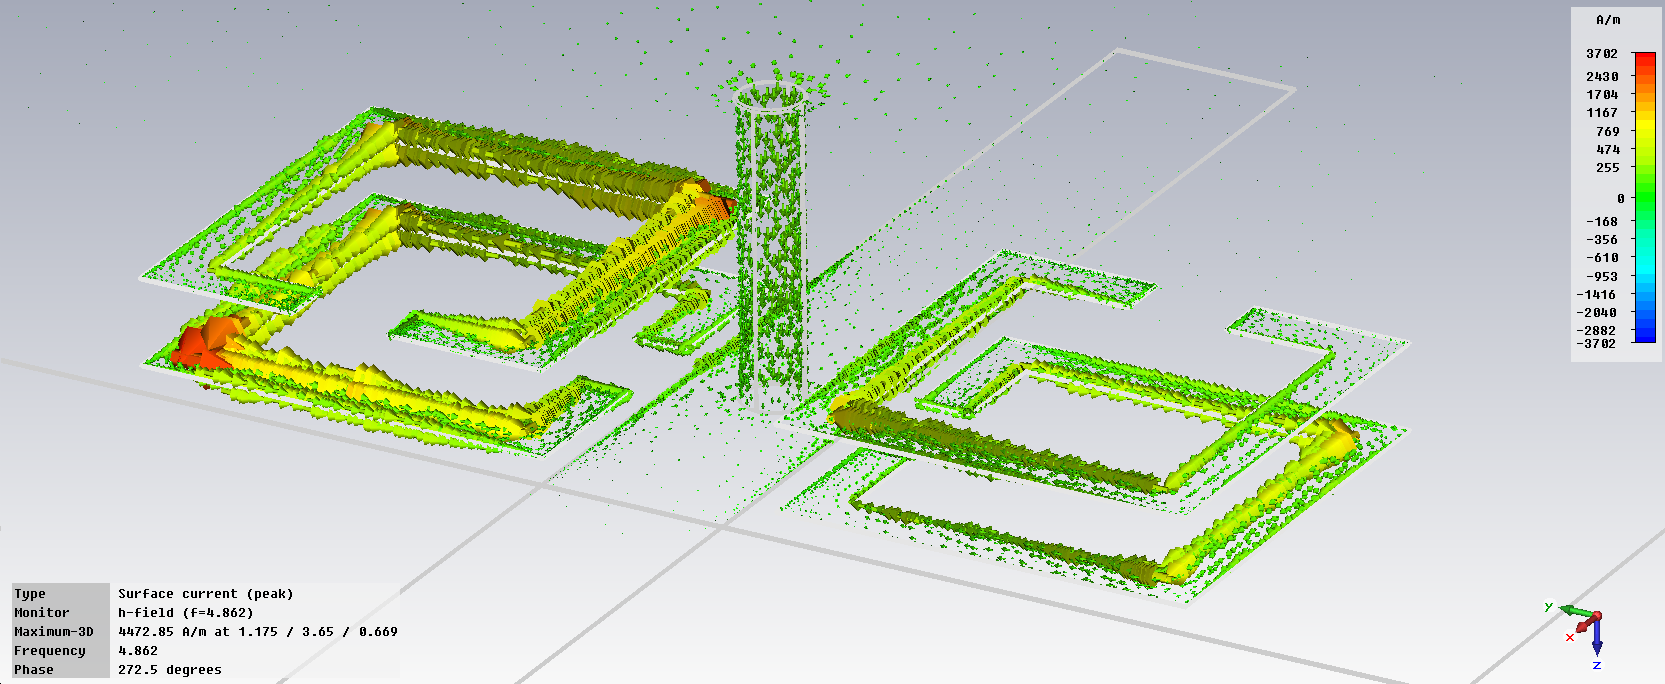
\includegraphics[width=1.0\linewidth]{sl_eit/str1.png}}\\
    \subfloat[]{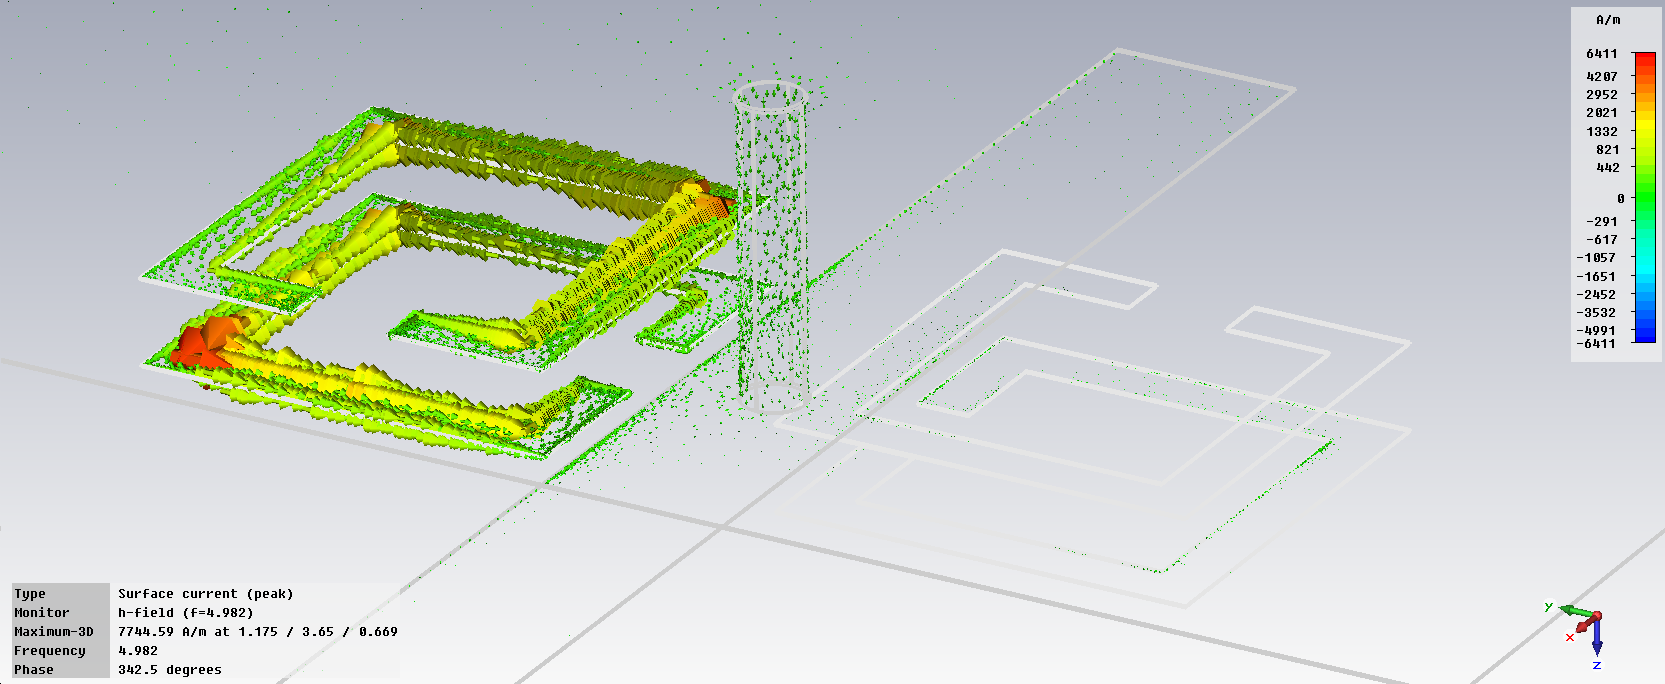
\includegraphics[width=1.0\linewidth]{sl_eit/str2.png}}\\
    \subfloat[]{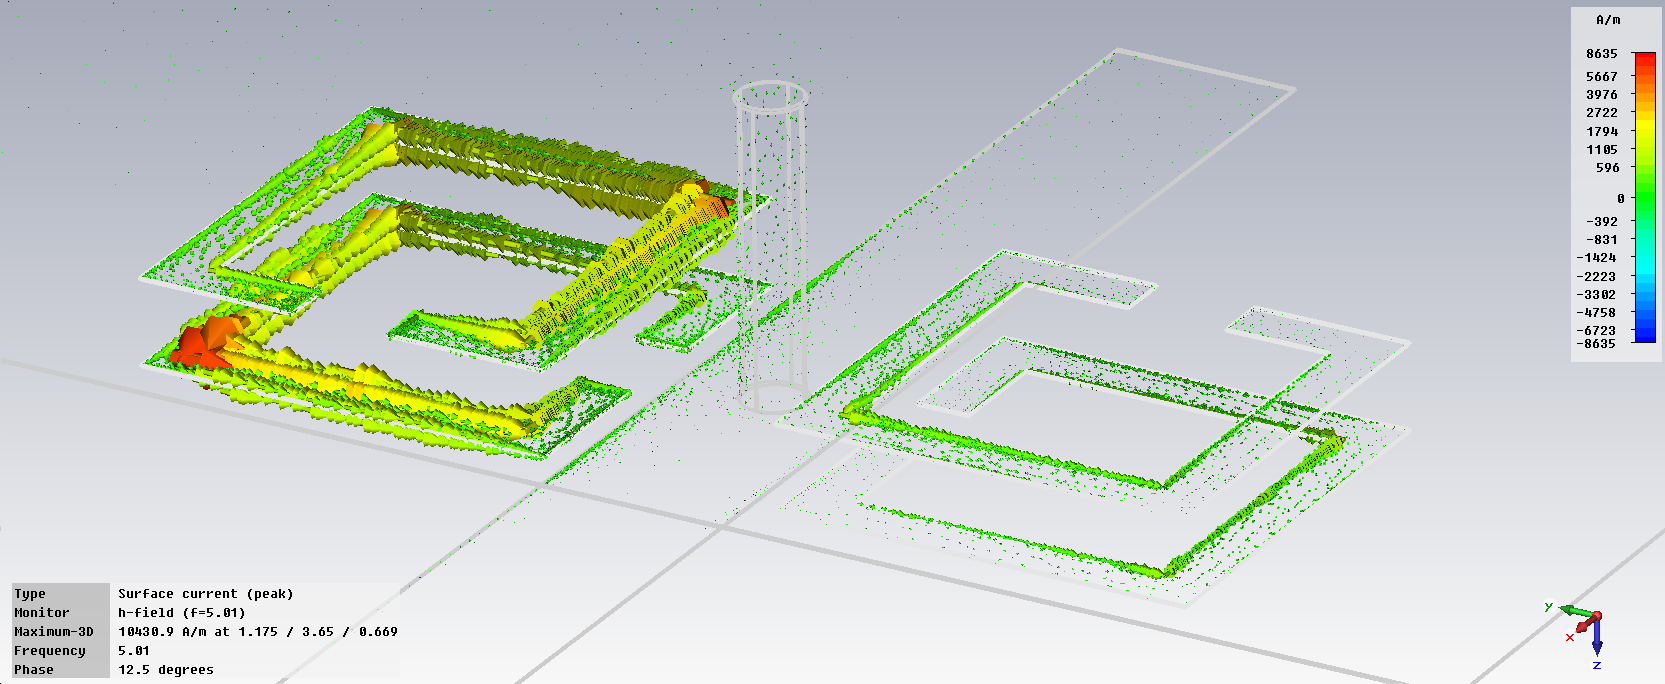
\includegraphics[width=1.0\linewidth]{sl_eit/str3.png}}\\
    \caption{Расподела струје на карактеристичним учестаностима.}
    \label{fig:sl_eit/str1}
\end{figure}
Како би се пружио додатни увид, расподела струје је прорачуната на карактеристичним фреквенцијама и приказана на сл.~\ref{fig:sl_eit/str1}. Са ње се види како је један пар прстенова потпуно непобуђен на фреквенцији, која одговара максимуму трансмисије, тј. да се понаша као „тамни`` елемент.

\section{Анализа помоћу теорије спрегнутих модова}%
\label{sec:analiza_pomotshu_teorije_spregnutikh_modova}

\begin{figure}[h]
    \centering
    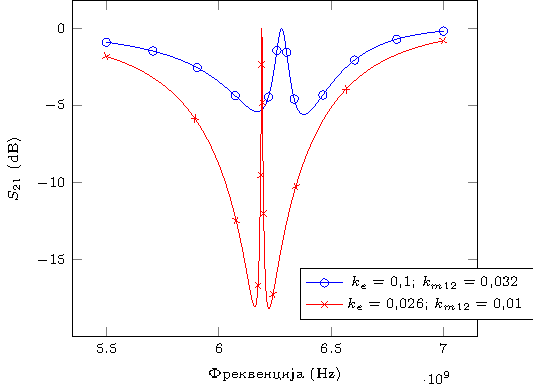
\includegraphics[width=0.8\linewidth]{sl_eit/etran.pdf}
    \caption{$L=\SI{1.47}{\nano\henry}$, $C=\SI{0.84}{\pico\farad}$, $L_S=\SI{7.91}{\nano\henry}$, $C_S=\SI{0.101}{\pico\farad}$ и $k_m=\num{0.3}$, док су преостале спреге дате у легенди.}
    \label{fig:sl_eit/etran}
\end{figure}
Недостатак структуре описане у претходној секцији је њена релативна сложеност, с обзиром да се састоји од укупно пет резонатора (четири прстена и вије). Од интереса је реализација класичног ЕИТ-а у једноставнијој структури, како би се олакшала анализа. Показује се да је ово могуће у случају структура из поглавља~\ref{ch:tsm}, које се састоје само од пара прстенова спрегнутих са водом~\cite{etran:2016}. Конкретно, коришћењем електричне шеме са сл.~\ref{tsm:sl3}, могуће је добити спектре приказане на сл.~\ref{fig:sl_eit/etran}, за вредности параметара дате у опису.

Предност коришћења ове структуре јесте то што је детаљно анализирана у глави~\ref{ch:tsm}, што се сада може искористити за тумачење. Наиме, пар спрегнутих прстенова поседује два резонантна мода, симетрични и антисиметрични, чији $Q$-фактори су дати изразима (\ref{tsm:eo_pom}). Одговарајућим подешавањем јачине електричне и магнетне спреге, могуће је остварити драстичну разлику у $Q$-факторима модова, уз истовремено преклапање резонантних учестаности. На овај начин се остварују раније наведени услови за класичну аналогију ЕИТ-а.

За разлику од механичког модела, теорија спрегнутих модова даје комплетнију слику, зато што може да опише не само међусобну спрегу резонатора, већ и њихову спрегу са водом. У том контексту, ефекат класичне аналогије ЕИТ-а се може тумачити као резултат ускопојасне деструктивне интерференције два резонантна мода на њиховом излазном порту.

Резултати са сл.~\ref{fig:sl_eit/etran} су рачунати не узимајући у обзир губитке. У пракси, показује се да укључивање губитака деградира приказани ефекат у значајној мери, у случају разматраних структура са сплит ринг резонаторима у микрострип технологији. У даљем истраживању планирано је испитивање других реализација, које би имале мање изражене губитке.

%\bibliographystyle{babplai3}
%\bibliography{ref}

\end{document}
